%%%%%%%%%%%%%%%%%%%%%%%%%%%%%%%%%%%%%%%%%%%%%%%
%%%     Declarations (skip to Begin Document, line 112, for parts you fill in)
%%%%%%%%%%%%%%%%%%%%%%%%%%%%%%%%%%%%%%%%%%%%%%%

\documentclass[10pt]{article}

\usepackage{geometry}  % Lots of layout options.  See http://en.wikibooks.org/wiki/LaTeX/Page_Layout
\geometry{letterpaper}  % ... or a4paper or a5paper or ... 
\usepackage{fullpage}  % somewhat standardized smaller margins (around an inch)
\usepackage{setspace}  % control line spacing in latex documents
\usepackage[parfill]{parskip}  % Activate to begin paragraphs with an empty line rather than an indent

\usepackage{amsmath,amssymb}  % latex math
\usepackage{empheq} % http://www.ctan.org/pkg/empheq
\usepackage{bm,upgreek}  % allows you to write bold greek letters (upper & lower case)

\usepackage{url}

% for typsetting algorithm pseudocode see http://en.wikibooks.org/wiki/LaTeX/Algorithms_and_Pseudocode
\usepackage{algorithmic,algorithm}  

\usepackage{graphicx}  % inclusion of graphics; see: http://en.wikibooks.org/wiki/LaTeX/Importing_Graphics
% allow easy inclusion of .tif, .png graphics
\DeclareGraphicsRule{.tif}{png}{.png}{`convert #1 `dirname #1`/`basename #1 .tif`.png}

\usepackage{xspace}
\newcommand{\latex}{\LaTeX\xspace}

\usepackage{color}  % http://en.wikibooks.org/wiki/LaTeX/Colors

\long\def\ans#1{{\color{blue}{\em #1}}}
\long\def\ansnem#1{{\color{blue}#1}}
\long\def\boldred#1{{\color{red}{\bf #1}}}

% Useful package for syntax highlighting of specific code (such as python) -- see below
\usepackage{listings}  % http://en.wikibooks.org/wiki/LaTeX/Packages/Listings
\usepackage{textcomp}

%%% The following lines set up using the listings package
\renewcommand{\lstlistlistingname}{Code Listings}
\renewcommand{\lstlistingname}{Code Listing}

%%% Specific for python listings
\definecolor{gray}{gray}{0.5}
\definecolor{green}{rgb}{0,0.5,0}

\lstnewenvironment{python}[1][]{
\lstset{
language=python,
basicstyle=\footnotesize,  % could also use this -- a little larger \ttfamily\small\setstretch{1},
stringstyle=\color{red},
showstringspaces=false,
alsoletter={1234567890},
otherkeywords={\ , \}, \{},
keywordstyle=\color{blue},
emph={access,and,break,class,continue,def,del,elif ,else,%
except,exec,finally,for,from,global,if,import,in,i s,%
lambda,not,or,pass,print,raise,return,try,while},
emphstyle=\color{black}\bfseries,
emph={[2]True, False, None, self},
emphstyle=[2]\color{green},
emph={[3]from, import, as},
emphstyle=[3]\color{blue},
upquote=true,
morecomment=[s]{"""}{"""},
commentstyle=\color{gray}\slshape,
emph={[4]1, 2, 3, 4, 5, 6, 7, 8, 9, 0},
emphstyle=[4]\color{blue},
literate=*{:}{{\textcolor{blue}:}}{1}%
{=}{{\textcolor{blue}=}}{1}%
{-}{{\textcolor{blue}-}}{1}%
{+}{{\textcolor{blue}+}}{1}%
{*}{{\textcolor{blue}*}}{1}%
{!}{{\textcolor{blue}!}}{1}%
{(}{{\textcolor{blue}(}}{1}%
{)}{{\textcolor{blue})}}{1}%
{[}{{\textcolor{blue}[}}{1}%
{]}{{\textcolor{blue}]}}{1}%
{<}{{\textcolor{blue}<}}{1}%
{>}{{\textcolor{blue}>}}{1},%
%framexleftmargin=1mm, framextopmargin=1mm, frame=shadowbox, rulesepcolor=\color{blue},#1
framexleftmargin=1mm, framextopmargin=1mm, frame=single,#1
}}{}
%%% End python code listing definitions

%%% Specific for matlab listings
\definecolor{dkgreen}{rgb}{0,0.6,0}
\definecolor{gray}{rgb}{0.5,0.5,0.5}
\definecolor{mauve}{rgb}{0.58,0,0.82}
 
\lstnewenvironment{matlab}[1][]{
\lstset{ %
  language=Matlab,                % the language of the code
  basicstyle=\footnotesize,           % the size of the fonts that are used for the code
  numbers=left,                   % where to put the line-numbers
  numberstyle=\tiny\color{gray},  % the style that is used for the line-numbers
  stepnumber=2,                   % the step between two line-numbers. If it's 1, each line 
                                  % will be numbered
  numbersep=5pt,                  % how far the line-numbers are from the code
  backgroundcolor=\color{white},      % choose the background color. You must add \usepackage{color}
  showspaces=false,               % show spaces adding particular underscores
  showstringspaces=false,         % underline spaces within strings
  showtabs=false,                 % show tabs within strings adding particular underscores
  frame=single,                   % adds a frame around the code
  rulecolor=\color{black},        % if not set, the frame-color may be changed on line-breaks within not-black text (e.g. commens (green here))
  tabsize=2,                      % sets default tabsize to 2 spaces
  captionpos=t,                   % sets the caption-position to top
  breaklines=true,                % sets automatic line breaking
  breakatwhitespace=false,        % sets if automatic breaks should only happen at whitespace
  title=\lstname,                   % show the filename of files included with \lstinputlisting;
                                  % also try caption instead of title
  keywordstyle=\color{blue},          % keyword style
  commentstyle=\color{dkgreen},       % comment style
  stringstyle=\color{mauve},         % string literal style
  escapeinside={\%*}{*)},            % if you want to add LaTeX within your code
  morekeywords={*,...}               % if you want to add more keywords to the set
  framexleftmargin=1mm, framextopmargin=1mm, frame=single,#1 % display caption
} }{}
%%% End matlab code listing definitions

%% hilite
\newcommand{\hilite}[1]{\colorbox{yellow}{#1}}
\long\def\todo#1{\hilite{{\bf TODO:} {\em #1}}}


%%%%%%%%%%%%%%%%%%%%%%%%%%%%%%%%%%%%%%%%%%%%%%%
%%%     Begin Document
%%%%%%%%%%%%%%%%%%%%%%%%%%%%%%%%%%%%%%%%%%%%%%%

\begin{document}

\begin{center}
    {\Large {\bf ISTA 421 / INFO 521 -- Homework 2}} \\
    \boldred{Due: Tuesday, Sept 21, 5pm} \\
    20 points total Undergraduate / 25 points total Graduate

\end{center}

\begin{flushright}
STUDENT NAME %% Fill in your name here

Undergraduate / Graduate %% select which you are!
\end{flushright}


\vspace{1cm}
{\Large {\bf Instructions}}

The purpose of this set of exercises is to demonstrate your ability to implement the generalized matrix form of the normal equations for linear regression, implement and use cross-validation, and gain experience interpreting simple regression results.

In this assignment you are required to write 2 scripts in python.  They will be submitted as 2 separate files, although you are free to copy any parts of code from one script to the next as desired.  The names for the script files are specified in problems 1 and 3 below.

Included in the homework 2 release are two sample scripts \\ 
\-\hspace{2cm}{\tt fitpoly.py} and {\tt cv.py} \\
and two data files\\
\-\hspace{2cm}{\tt womens100.csv}, and {\tt synthdata2021.csv}\\

The sample scripts are provided for your convenience -- you may use any part of the code in those scripts for your submissions.  Note that neither will run just as provided: you must fill in the calculation of $\mathbf{w}$.  The data files are provided in {\tt .csv} (comma separated values) format.  The script {\tt fitpoly.py} contains the function {\tt read\_data} which shows how to load the data files into a numpy array.

All exercises after Exercise 1 require that you provide some ``written'' answers.  In some of these, you must also include figures; remember that you {\bf must} always label any figure axes and include an informative figure caption with each figure.  You will submit a PDF of your written answers.  (You can use \latex or any other system (including handwritten; plots, of course, must be program-generated) as long as the final version is in PDF and any handwritten answers MUST be legible or we will not grade it.)

The final submission will include (minimally) the two scripts and a PDF version of your written part of the assignment. You submitted PDF written answers must be named {\tt hw3-answers.pdf}.

NOTE: Problems 4 and 5 are required for Graduate students only; Undergraduates may complete them for extra credit equal to the point value.

FCML refers to the course text: Rogers and Girolami (2016), {\em A First Course in Machine Learning, Second Edition}.  

For general notes on using \latex to typeset math, see: {\tt http://en.wikibooks.org/wiki/LaTeX/Mathematics}
\vspace{.5cm}

%%%%%%%%%%%%%%%%
%%%     Problems
%%%%%%%%%%%%%%%%

\newpage
\begin{itemize}



%%% START Exercise 1 %%%
\item[1.] [5 points]
Adapted from {\bf Exercise 1.2} of FCMA p.35:

In this exercise you will complete the implementation of the function {\tt fitpoly} in {code/fitpoly.py} so that it can compute the best-fit parameters $\mathbf{w}$ (a vector of parameters) for a linear model with one feature per observation. After you have implemented {\tt fitpoly}, you can complete the implementation of the function {\tt exercise\_1} to fit to the Women's 100 meter dash data.

{\tt fitpoly} takes as input an array, {\tt x}, representing all of the feature observations, and the array {\tt t} representing the corresponding response values. The elements at index 0 of {\tt x} and {\tt t} together represent the first feature/response ``training'' pair, index 1 of {\tt x} and {\tt t} represents the second ``training'' pair, etc.

{\tt fitpoly} is used in {\tt exercise\_1} to only fit a simple line to the data (i.e., you only need to fit parameters $w_0$ and $w_1$). However, in the in later exercises (such as Exercise 2) you will need to fit higher-order polynomial models (e.g., $t = w_0 + w_1x + w_2x^2 + ...$). For this reason, you must make your implementation of {\tt fitpoly} generalized to handle higher-order polynomials. 

The parameter {\tt model\_order} is used in {\tt fitpoly} to represent the non-negative integer, $n$, that in turn represents the highest order polynomial exponent of the polynomial model:
\begin{eqnarray*}
t = w_0 x^0 + w_1 x^1 + w_2 x^2 + ... + w_n x^n
\end{eqnarray*}

The implementation of {\tt fitpoly} starts with a construction of the {\em design matrix}, $\mathbf{X}$: the representation of input features as a matrix, where each row in the matrix corresponds to an individual observation and the columns represent the features for each individual. See the provided comments in {\tt fitpoly} for an explanation of how the design matrix $\mathbf{X}$ is represented.

Your first task in this exercise is to implement the matrix normal equations to compute the parameter vector $\mathbf{w}$ (3\$).

Note: the {\tt fitpoly.py} file includes three helper functions (Utilities) to read data, plot data, and plot the model (once you've determined the weight vector $\mathbf{w}$), but the function for computing linear least-squares fit is {\em incomplete}.  {\tt fitpoly} takes as input the (one-dimensional) data vector $\mathbf{x}$, the target values vector $\mathbf{t}$, and a non-negative integer {\tt model\_order}, which represents the highest polynomial order term of the model; {\tt fitpoly} is intended to return the $\mathbf{w}$ vector (as a numpy array).

Remember: the Appendix to HW 1 has a brief tutorial on working with numpy arrays.

{\bf Just to state the obvious}: the objective of this exercise is for you to implement the linear least squares fit solution (i.e., the normal equation) in its general linear algebra form.  {\bf DO NOT} use existing least squares solvers, such as {\tt numpy.linalg.lstsq}, or scikit learn's \\{\tt sklearn.linear\_model.LogisticRegression} as your implemented solution; however, it is certainly fine to use those functions to help you {\em verify} your implementation's output (but don't submit those as your solution).

You can now test your implementation of {\tt fitpoly} by completing the implementation of the {\tt exercise\_1} function. Table 1.3 (p.13) of FCMA lists the women's 100m gold medal Olympic results -- this data is provided in the file {\tt womens100.csv} in the {\tt data} folder. Use the provided function {\tt read\_data\_fit\_plot} to find the 1st-order polynomial model (i.e., a line with parameters $w_0$ and $w_1$) that minimizes the squared loss of this data. (Note that the call of {\tt exercise\_1} by the TOP LEVEL SCRIPT at the bottom of the file will already provide the path to the data file; you need to fill in the rest of the parameters to {\tt read\_data\_fit\_plot}). Choose parameters to {\tt read\_data\_fit\_plot} to save your plot figure in the {\tt figures} directory. Report the model here as an equation (e.g., $t = 2 + 4x \leftarrow$ that is just an example); you only need to report parameter values up to 3 decimal places.  Plot the data with your best-first model and include the plot in your answer (label axes and include an informative caption!) (2\$).

{\bf Solution.} 
%%% For latex users: code to insert figure
%\begin{figure}[htb]
%\begin{center}
%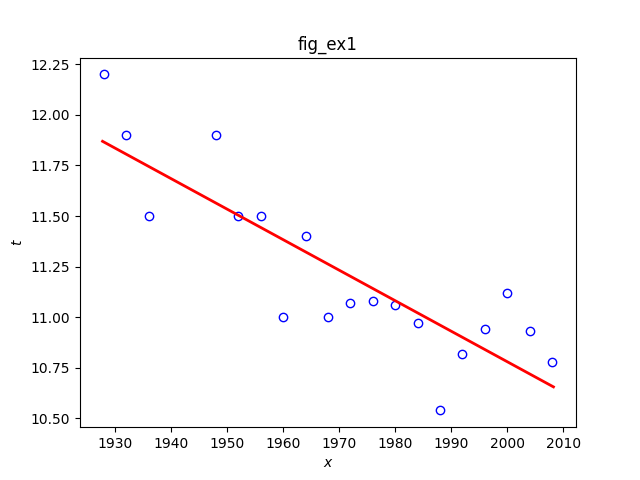
\includegraphics[width=8cm]{figures/womens100-best-fit}
%\ans{\caption{YOUR CAPTION HERE{fig:womens100}}}
%\end{center}
%\end{figure}
%%% END Exercise 1 %%%



%%% START Exercise 2 %%%
\item[2.] [3 points]
Adapted from {\bf Exercise 1.9} of FCMA p.36:

Now fill in {\tt exercise\_2} similar to {\tt exercise\_1}, but this time you will load the data stored in the file {\tt synthdata2021.csv} (in the data folder) and fit a 3rd order polynomial function -- $f(x; \mathbf{w}) = w_0 + w_1 x + w_2 x^2 + w_3 x^3$ -- to this data. There are 25 observations in this data.
Report the best-fit model parameters as an equation. Plot the data and your model and include the plot in your answer (be sure to include an informative caption to your plot).

{\bf Solution.} 
%%% For latex users: code to insert figure
%\begin{figure}[htb]
%\begin{center}
%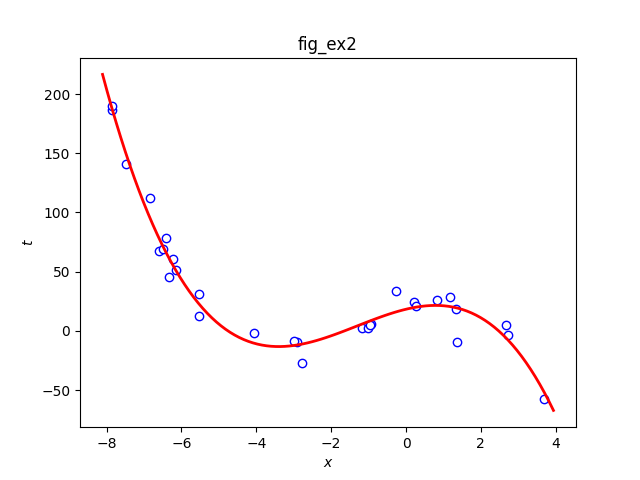
\includegraphics[width=8cm]{figures/synthetic2021-3rd-poly.png}
%\ans{\caption{YOUR CAPTION HERE\label{fig:synth3rd}}}
%\end{center}
%\end{figure}
%%% END Exercise 2 %%%



%%% START Exercise 3 %%%
\item[3.] [12 points]
The script {\tt code/cv.py} is an {\em almost complete} implementation of the demonstration in Chapter 1 of FCML, pp.31-32, of cross-validation. In the demonstration, CV is used to assess the best fit of polynomial models across different polynomial model orders given only 30 total observations. In the demo, the code also contrasts the cross-validation results with results from an {\em independent} set of data (sampled from the {\em same} data generating process) that is significantly larger (in this case, $1000$ observations).

The purpose of this demonstration is both to show an example of how cross-validation for model search is implemented, and to show that even though cross-validation might work with a very small data set (in this case, $30$ observations), its results are similar to evaluating with much more data ($1000$ observations). Read the description in Ch. 1 and make sure you understand how this has been implemented in the code. 

The core of the implementation is in the functions {\tt run\_cv} and {\tt run\_demo}. The global variable {\t RUN\_DEMO} is a boolean that controls whether the demo is run (by default this is set to {\tt True}, on line 26 of {\tt code/cv.py}). 

I say that this is an {\em almost complete} implementation because it is missing one step: the calculation of the best-fit values for $\mathbf{w}$. You will need to fill this in yourself at the indicated location in {\tt run\_cv} (\$). The calculation here should be the same solution you used for calculating {\tt w} in {\tt fitpoly} in Exercise 1. Before you implement this, when you run the script, it will generate one plot (of the generated data) and print the following two lines to the terminal:
\begin{verbatim}
run_demo(): best_polynomial model order: None
run_demo(): min_mean_log_cv_loss: None
\end{verbatim}

Once you have filled in the calculation of {\tt w}, then when you run the demo, it will generate two figures, and the best polynomial model order and the minimum log cv loss (explained below) will no longer be printed to the terminal as {\tt None}.

The first figure generated by the demo shows a plot of the synthetically-generated $30$ data points (blue circles) used for cross-validation; the green line represents the function (the mean of the ``generating process'') from which these were sampled (the $*$ on the $t$ indicates that these are response values of $t$ from the ``true'' function):
\begin{eqnarray*}
t^* = x + 5x^2 + 2x^3
\end{eqnarray*}
The random samples (blue circles) consist of $x$ values uniformly randomly sampled between $-5$ and $5$, and $t$ sampled from a Gaussian (Normal) distribution with mean $t^*$ and standard deviation {\tt sigma}: $\mathcal{N}(t^*, \mathrm{\tt sigma})$.

The second figure shows three plots of the log mean squared error (MSE) of the loss as the polynomial order of the model varies from $0$ to $7$. The first plot is the log MSE loss of the models on the training data. As this is cross-validation, this is the {\em mean} loss across each of the fold training data. In {\tt run\_demo} you can see the number of folds, {\tt K}, is set to $10$, so this is 10-fold cross-validation. Because we have a total of $30$ data points, and $K=10$, then the training set of each fold will have $27$ data points, and the CV Train Loss will be assessed for fit on the $27$ data points in each fold training set; there are $10$ such training loss calculations (one for each fold), so the reported mean in the first plot is then the (log) mean of those $10$ losses based on the CV training sets. The second plot shows the log MSE loss for each model order where the CV Test Loss is now computed based on the $3$ held-out data points within each fold, and there are $10$ such folds, so the mean is across those $10$ losses. Finally, the third plot shows the log MSE loss on the completely independent test dataset (still generated from the same ``true'' function) consisting of $1000$ data points, so the mean loss (for each model order) is based on the model fit to the $1000$ points in the independent test set. As can be seen, the Independent Test and CV Test loss are both similar U-shaped curves, and there is a trend toward a minimum loss around model order 3 (which happens to be the order of the polynomial used to generate both the CV and independent test set data). The CV Train Loss, however, keeps getting smaller as the model order increases, because the model is getting to fit to exactly the same data used to report the loss, and in general as the model order increases, it will fit better to that data due to increased flexibility of the model (given its higher order polynomial flexibility).

Note that the first step in the top-level {\tt run\_demo} function is to set the random seed (as you did in Homework 1), and the call to {\tt run\_demo} in the TOP LEVEL SCRIPT by default sets this to $29$. This makes it so that each time you execute the script, you get the same results, even though you are sampling from the random number generator. If you change the random seed, you will get different behavior, which is expected. Give it a try! You'll see that some times the CV and Independent Test Losses don't always have a minimum at model order 3. And some times the CV Test and Independent Test loss across model orders can go up and then down again.

Now to the main task. In this Exercise, you are tasked with implementing K-fold cross-validation to perform model selection, in this case to search for the model of polynomial order (between orders 0 and 7) with the best predictive error for the data in {\tt data/synthdata2021.csv}. You can use and adapt any part of implementation of the demo. A key difference is that unlike the demo, you are working with the given data in {\tt data/synthdata2021.csv}, so {\bf you will {\em not} be generating your own synthetic data, and there will {\em not} be an independent test set of data} -- you will just focus on implementing straight cross-validation (with its train and test data splits within each fold), without the {\em additional} independent test set.

You will need to run your implementation under two conditions: 5-fold cross-validation, to be performed in the function {\tt exercise\_3\_5fold}, and Leave-One-Out cross-validation (LOOCV), to be performed in the function {\tt exercise\_3\_LOOCV}. It is recommended (but not necessary) that you create a single function that can run your cross-validation experiment and return the needed values, so that you don't have to repeat a lot of code between {\tt exercise\_3\_5fold} and {\tt exercise\_3\_LOOCV}.

For both cases (again, possibly by a call to a single function), you are asked to {\em randomize} the order of your data. Although the demo does not do this by default, it includes code to show you how you can randomize the order of the data before you then perform your cross-validation. The reason for asking you to do this here is that as long as you are not working with data that has a natural order dependency (such as time series), it good general good practice to randomize, especially if you are not sure that the order of your data has already been randomized. In this case, the data is independent data, so it is good to randomize. If the order is not randomized, then the estimate of the generalization error being made by cross-validation could be biased. Because we still want to allow for reproducibility (this helps automating grading), set the random seed to 29 before you proceed with your randomization.

In both {\tt exercise\_3\_5fold} and {\tt exercise\_3\_LOOCV}, based on your cross-validation results, find and report the following in your written solution:
\begin{enumerate}
\item The polynomial model order that was found to fit best overall to the synthetic data,
\item The log mean squared error (MSE) for the CV Test data of that best-fit model order (i.e., for that best-fit model, calculating the loss on each of the held-out test data in each fold, and reporting the mean across the folds).
\item The model parameters for the best fit model of the best-fit model order
\end{enumerate}

A pytest unit test is provided to test the results of Exercise 3 (for both {\tt exercise\_3\_5fold} and {\tt exercise\_3\_LOOCV}) against the results that I get in my reference implementation. HOWEVER, note that because there are many different ways that you might end up calling the random number generator, and thus affecting the outcome, you may have a correct implementation and yet these tests still fail. The tests are provided as a guide to help you know when you have a definite solution, but if they are not passing, that does not mean you do not have a viable solution. I wish there was a way to provide a more "relaxed" guide to tell you when you have achieved {\em some} viable solution, but unfortunately that is not possible to fully automate.

Finally, for {\tt exercise\_3\_5fold} and {\tt exercise\_3\_LOOCV}, you must also generate plots of the cross-validation results, similar to what is done in the demo, showing the CV Training log MSE loss, and the CV Test log MSE loss, across the 8 different polynomial model orders: 0..7. In total,  this means you will provide the following: (1) 5-fold CV Training with (2) related Test loss, and (3) LOOCV Training, and (4) Test loss. NOTE: You can use the provided {\tt plot\_cv\_results} function to plot the just the CV Training and CV Test loss (whether 5-fold or LOOCV) as a pair of plots -- in this case, if you pass the value {\tt None} to the argument for {\tt ind\_loss}, the function will skip rendering the third ``independent test'' plot (this was used in the demo). In hw2, you must save these figures to the `{\tt figures}' directory, and also include them in your PDF submission (this means you must add, commit and push them in your final submission).

If you use {\tt plot\_cv\_results}, save your figures as follows:
\begin{itemize}
\item For 5-fold CV, save the combined plots in `{\tt figures/synthetic2021-5fold-CV.png}'
\item For LOOCV, save the combined plots in `{\tt figures/synthetic2021-LOOCV.png}'
\end{itemize}
There is again a unit test to test whether these plots have been generated. If you instead generated the plots under a different name, the unit tests will fail, but as long as you create the plots and include then in your written PDF submission, you will get full credit.

{\bf Solution.} 

%%% END Exercise 3 %%%



%%% START Exercise 4 %%%
\item[4.] [2 points -- {\bf Required only for Graduates}] 
{\bf Exercise 1.10} from FCMA p.36

Derive the optimal least squares parameter value, $\mathbf{\hat{w}}$, for the total training loss:
\begin{eqnarray*}
\mathcal{L} = \sum_{n=1}^N \left( t_n - \mathbf{w}^\top \mathbf{x}_n \right)^2
\end{eqnarray*}

How does the expression compare with that derived from the average (mean) loss?  (Hint: Express this loss in the {\bf full} matrix form and derive the normal equation.)

{\bf Solution.} 

%%% END Exercise 4 %%%



%%% START Exercise 5 %%%
\item[5.] [3 points -- {\bf Required only for Graduates}]
{\bf Exercise 1.11} from FCMA p.36

The following expression is known as the {\em weighted} average loss:
\begin{eqnarray*}
\mathcal{L} = {1 \over N} \sum_{n=1}^N \alpha_n \left( t_n - \mathbf{w}^\top \mathbf{x}_n \right)^2
\end{eqnarray*}

where the influence of each data point is controlled by its associated parameter.  Assuming that each $\alpha_n$ is fixed, derive the optimal least squares parameter value $\mathbf{\hat{w}}$.  (Hint: When expressing in the full matrix form, the $alpha$'s become a matrix...)

{\bf Solution.} 

%%% END Exercise 5 %%%


\end{itemize}

\end{document}